%%%%%%%%%%%%%%%%%%%%%%%%%%%%%%%%%%%%%%%
% Wenneker Resume/CV
% LaTeX Template
% Version 1.1 (19/6/2016)
%
% This template has been downloaded from:
% http://www.LaTeXTemplates.com
%
% Original author:
% Frits Wenneker (http://www.howtotex.com) with extensive modifications by 
% Vel (vel@LaTeXTemplates.com)
%
% License:
% CC BY-NC-SA 3.0 (http://creativecommons.org/licenses/by-nc-sa/3.0/
%
%%%%%%%%%%%%%%%%%%%%%%%%%%%%%%%%%%%%%%

%----------------------------------------------------------------------------------------
%	PACKAGES AND OTHER DOCUMENT CONFIGURATIONS
%----------------------------------------------------------------------------------------

\documentclass[a4paper,10pt]{memoir} % Font and paper size

%%%%%%%%%%%%%%%%%%%%%%%%%%%%%%%%%%%%%%%%%
% Wenneker Resume/CV
% Structure Specification File
% Version 1.1 (19/6/2016)
%
% This file has been downloaded from:
% http://www.LaTeXTemplates.com
%
% Original author:
% Frits Wenneker (http://www.howtotex.com) with extensive modifications by 
% Vel (vel@latextemplates.com)
%
% License:
% CC BY-NC-SA 3.0 (http://creativecommons.org/licenses/by-nc-sa/3.0/)
%
%%%%%%%%%%%%%%%%%%%%%%%%%%%%%%%%%%%%%%%%%

%----------------------------------------------------------------------------------------
%	PACKAGES AND OTHER DOCUMENT CONFIGURATIONS
%----------------------------------------------------------------------------------------

\usepackage{lato} % Use the Bitstream Charter font
\usepackage[utf8]{inputenc} % Required for inputting international characters
\usepackage[T1]{fontenc} % Output font encoding for international characters

\usepackage[top=2cm,left=1cm,right=1cm,bottom=2cm]{geometry} % Modify margins

\usepackage{graphicx} % Required for figures

\usepackage{flowfram} % Required for the multi-column layout

\usepackage{url} % URLs
\usepackage{hyperref}

\usepackage[usenames,dvipsnames]{xcolor} % Required for custom colours

\usepackage{tikz} % Required for the horizontal rule

\usepackage{enumitem} % Required for modifying lists
\setlist{noitemsep,nolistsep} % Remove spacing within and around lists

\setlength{\columnsep}{\baselineskip} % Set the spacing between columns

% Define the left frame (sidebar)
\newflowframe{0.2\textwidth}{\textheight}{0pt}{0pt}[left]
\newlength{\LeftMainSep}
\setlength{\LeftMainSep}{0.2\textwidth}
\addtolength{\LeftMainSep}{1\columnsep}
 
% Small static frame for the vertical line
\newstaticframe{1.5pt}{\textheight}{\LeftMainSep}{0pt}
 
% Content of the static frame with the vertical line
\begin{staticcontents}{1}
\hfill
\tikz{\draw[loosely dotted,color=RoyalBlue,line width=1pt,yshift=0](0,0) -- (0,\textheight);}
\hfill\mbox{}
\end{staticcontents}
 
% Define the right frame (main body)
\addtolength{\LeftMainSep}{1.5pt}
\addtolength{\LeftMainSep}{1\columnsep}
\newflowframe{0.7\textwidth}{\textheight}{\LeftMainSep}{0pt}[main01]

\pagestyle{empty} % Disable all page numbering

\setlength{\parindent}{0pt} % Stop paragraph indentation

%----------------------------------------------------------------------------------------
%	NEW COMMANDS
%----------------------------------------------------------------------------------------

\newcommand{\userinformation}[1]{\renewcommand{\userinformation}{#1}} % Define a new command for the CV user's information that goes into the left column

\newcommand{\cvheading}[1]{{\Huge\bfseries\color{RoyalBlue} #1} \par\vspace{.6\baselineskip}} % New command for the CV heading
\newcommand{\cvsubheading}[1]{{\Large\bfseries #1} \bigbreak} % New command for the CV subheading

\newcommand{\Sep}{\vspace{0.8em}} % New command for the spacing between headings
\newcommand{\SmallSep}{\vspace{0.5em}} % New command for the spacing within headings

\newcommand{\aboutme}[2]{ % New command for the about me section
\textbf{\color{RoyalBlue} #1}~#2\par\Sep
}
	
\newcommand{\CVSection}[1]{ % New command for the headings within sections
{\Large\textbf{#1}}\par
\SmallSep % Used for spacing
}

\newcommand{\CVItem}[3]{ % New command for the item descriptions
\textbf{\color{RoyalBlue} #1 \hfill {#2}}
\par
#3
\SmallSep % Used for spacing
}

\newcommand{\bluebullet}{\textcolor{RoyalBlue}{$\circ$}~~} % New command for the blue bullets
 % Include the file specifying document layout and packages

%----------------------------------------------------------------------------------------
%	NAME AND CONTACT INFORMATION 
%----------------------------------------------------------------------------------------

\userinformation{ % Set the content that goes into the sidebar of each page
\begin{flushright}
% Comment out this figure block if you don't want a photo
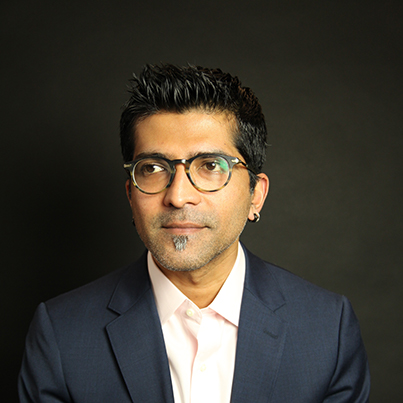
\includegraphics[width=0.6\columnwidth]{shameel_portrait_2017_small.jpg}\\[\baselineskip] % Your photo
\small % Smaller font size
Shameel Arafin \\ % Your name
shameel@arafin.net \\ % Your email address
@algebraist \\ % Your URL
(215) 982-0854 \\ % Your phone number
\Sep % Some whitespace
\textbf{Address} \\
469A Lexington Ave, \#1 \\ % Address 1
Brooklyn, NY 11221 \\ % Address 2
% United States \\ % Address 3
\vfill % Whitespace under this block to push it up under the photo
\end{flushright}
}

%----------------------------------------------------------------------------------------

\begin{document}

\userinformation % Print your information in the left column

\framebreak % End of the first column

%----------------------------------------------------------------------------------------
%	HEADING
%----------------------------------------------------------------------------------------

\cvheading{Shameel Arafin} % Large heading - your name

% \cvsubheading{Technology Executive} % Subheading - your occupation/specialization

%----------------------------------------------------------------------------------------
%	ABOUT ME
%----------------------------------------------------------------------------------------

\aboutme{Technology Executive}{with extensive domain expertise in media, focused on digital journalism, documentary and online learning. Results-driven leader, mentor, engineering gender-parity advocate. 10+ years in web development, product management and project development.}

%----------------------------------------------------------------------------------------
%	EXPERIENCE
%----------------------------------------------------------------------------------------

\CVSection{Experience}

%------------------------------------------------

\CVItem{Meredith Corp./formerly Time Inc.}{April 2017 - February 2018}{\textit{Senior Director, Platform Engineering, News Group}}
\begin{itemize}
	\item Successfully launched multiple award-winning projects, including  \href{http://time.com/time-person-of-the-year-2017-silence-breakers/}{TIME's Person of the Year ``The Silence Breakers"} and \href{http://time.com/finding-home/}{``Finding Home"}, winner of American Society of Magazine Editors (ASME) and Picture of the Year (POY) awards, Emmy-nominated.
	\item Launched News and Health brands' second redesign and and \href{https://medium.com/@acharalambides/element-the-digital-unification-of-time-inc-979656149fd3}{re-platforming to Element} (proprietary front-end platform).
	\item Recruited and led over a dozen developers, growing a team from 2 to 14 members, whose composition approached gender parity (43\% female).
	\item Expanded purview to include \href{http://www.health.com}{Health} vertical and all Foundry brands (the company's internal ad agency), as well as branded content/native advertising efforts. Managed multimillion-dollar engagements, working closely with advertising and marketing teams.
	\item Deeply involved in mentoring throughout the company, in Product, Design and Engineering departments. 
\end{itemize}
\Sep % Extra whitespace after the end of a major section

%------------------------------------------------

\CVItem{Time Inc.} {August 2015 - April 2017}{\textit{Director, Platform Engineering, News Group}}
\begin{itemize}
	\item Led engineering team for News and Education verticals, responsible for all technological aspects of \href{http://time.com}{time.com}, \href{http://fortune.com}{fortune.com},  \href{http://money.com}{money.com}, \href{https://www.timeforkids.com}{timeforkids.com}. 
	\item Successfully re-launched iconic franchises such as \href{http://fortune.com/fortune500}{FORTUNE 500}, \href{http://time.com/time-person-of-the-year-2017-silence-breakers/}{Person of the Year}, \href{http://time.com/collection/most-influential-people-2018/}{TIME 100 Most Influential People}.
	\item Drove re-architecture, re-platforming and development of \href{https://www.timeforkids}{Time For Kids}, from simple Drupal-based CMS to sophisticated WordPress VIP-powered learning management system. Features included multiple lexile levels, Spanish translations, audio read-aloud of text, and online-assessment and testing software.
	\item Managed redesign and re-platforming efforts for all News brands to headless WordPress VIP architecture, including Node/Express/React-powred front-end.
	\item Supervised engineering team for native/branded content engagements for The Foundry, for clients including \href{http://time.com/paid-content-from/netflix/dinnertime/}{Netflix} and \href{http://time.com/partner/siemens/innovation-starts-here/}{Siemens} (seven-figure engagement).
\end{itemize}
\Sep % Extra whitespace after the end of a major section

%------------------------------------------------
\CVItem{MediaStorm}{June 2011 - July 2015}{\textit{Platform Architect \& Lead Developer}}
\begin{itemize}
	\item Created architecture and back-end development for MediaStorm Platform, an interactive storytelling tool. 
	\item First online video player to \href{http://time.com/46716/game-changer-mediastorm-launches-pay-per-story-video-player/}{implement transaction (pay to view)}, built on proprietary CMS. Key users/clients include \href{https://mediastorm.com/clients/2018-icp-infinity-awards}{Wall Street Journal's Infinity Awards}, \href{https://mediastorm.com/clients/sundance-short-film-challenge}{Sundance Institute}, \href{https://mediastorm.com/clients/i-am-not-who-they-think-i-am-for-ictj}{International Center for Transitional Justice}. 
	\item Led technology sections for MediaStorm Workshops.
	\item Recruited developers and interns. Initiated 401(k) plan.
\end{itemize}
\Sep % Extra whitespace after the end of a major section

%------------------------------------------------
\CVItem{Freelance Engagements}{January 2003 - June 2011}{\textit{CTO, Lead Developer}}
\begin{itemize}
	\item PopStay: Architected and coded prototype of social app for vacation rentals and home swapping.
	\item Co-founded SignalFive, an interactive design, development and strategy agency for web/mobile apps. Clients included Al Gore's Alliance for Climate Protection and Grand Marnier. 
	\item Massify: Back-end developer at startup social network/crowd-sourcing web application for the film and TV industry.
\end{itemize}
\Sep % Extra whitespace after the end of a major section

\clearpage % Start a new page
\userinformation % Print your information in the left column
\framebreak % End of the first column


%------------------------------------------------

\CVItem{Credit Suisse First Boston Tech Group}{July 1998 - March 2002}{\textit{Senior Research Associate}}
\begin{itemize}
	\item Equity research in Semiconductor Capital Equipment and Communications Test \& Measurement sectors
\end{itemize}
\Sep % Extra whitespace after the end of a major section

%------------------------------------------------
\CVItem{Deutsche Bank Securities Tech Group}{June 1997 - July 1998}{\textit{Research Assistant}}
\begin{itemize}
	\item Research Assistant to Director of Research/Lead Analyst on PC Hardware \& Software 
	\item Editor of \textit{The Tech Daily}
\end{itemize}

\Sep % Extra whitespace after the end of a major section

%----------------------------------------------------------------------------------------
%	MENTORSHIP/TEACHING
%----------------------------------------------------------------------------------------

\CVSection{Mentorship/Teaching/Advisory}

%------------------------------------------------

\CVItem{CUNY 2X Tech}{Summer 2017 - Present}{\textit{Working Group Advisor}}
\begin{itemize}
	\item CUNY colleges computer science departments syllabus advisory 
	\item Working Group panelist and member
\end{itemize}

\Sep % Extra whitespace after the end of a major section

\CVItem{High School of Art \& Design}{November 2016 - Present}{\textit{Advisory Board Member}}
\begin{itemize}
	\item Syllabus ratification per New York Department of Education 
	\item Portfolio reviews, guest speaking
\end{itemize}

\Sep % Extra whitespace after the end of a major section


\CVItem{Mountain Workshops, Western Kentucky University}{October 2017}{\textit{Digital Storytelling \& Data Visualization Coach}}
\begin{itemize}
	\item Co-led weeklong workshop with half a dozen students, using code, design, photo, video, cartography and mapping to tell local stories
\end{itemize}

%------------------------------------------------

\Sep % Extra whitespace after the end of a major section

%----------------------------------------------------------------------------------------
%	Certifications
%----------------------------------------------------------------------------------------

\CVSection{Certifications}

%------------------------------------------------

\CVItem{Scrum Alliance}{February 2018 - Present}{\textit{Certified Scrum Product Owner}}
\Sep % Extra whitespace after the end of a major section


%----------------------------------------------------------------------------------------
%	EDUCATION
%----------------------------------------------------------------------------------------

\CVSection{Education}

%------------------------------------------------

\CVItem{Harvard University}{September 1995 - June 1997}{A.B. Literature (Honors)}

%------------------------------------------------

\CVItem{California Institute of Technology}{September 1993 - June 1995}{Electrical Engineering / Literature candidate}

%------------------------------------------------

\Sep % Extra whitespace after the end of a major section

%----------------------------------------------------------------------------------------
%	SKILLS
%----------------------------------------------------------------------------------------

% \CVSection{Technical Skills}

%------------------------------------------------
% {\begin{tabular}{p{0.2\textwidth} p{0.2\textwidth} p{0.2\textwidth}}
% 	\bluebullet Python/Django &
% 	\bluebullet Node/Express &
% 	\bluebullet PHP/CodeIgniter\\
	
% 	\bluebullet Postgresql/MySQL &  
 % 	\bluebullet AWS &  
 % 	\bluebullet WordPress VIP\\
% \end{tabular}}
% \Sep % Extra whitespace after the end of a major section

%------------------------------------------------

%----------------------------------------------------------------------------------------
%	NEW PAGE DELIMITER
%	Place this block wherever you would like the content of your CV to go onto the next page
%----------------------------------------------------------------------------------------

% \clearpage % Start a new page
% \userinformation % Print your information in the left column
% \framebreak % End of the first column

%----------------------------------------------------------------------------------------
%	AWARDS
%----------------------------------------------------------------------------------------

% \CVSection{Awards}

%------------------------------------------------

% \CVItem{2010, \textit{Postgraduate Scholarship}, Cornell University}{Awarded to the top student in their final year of a Bachelors degree.}

%------------------------------------------------

% \Sep % Extra whitespace after the end of a major section

%----------------------------------------------------------------------------------------
%	INTERESTS
%----------------------------------------------------------------------------------------

\CVSection{Interests}

%------------------------------------------------

\begin{itemize}
	\item Digital publishing, digital journalism 
	\item Interactive storytelling, documentary video, digital design
	\item Trail running, photography
\end{itemize}

\Sep % Extra whitespace after the end of a major section

%----------------------------------------------------------------------------------------

\end{document}
